\documentclass[letterpaper]{article}
\usepackage[margin=1in]{geometry}
\usepackage[utf8]{inputenc}
\usepackage{textcomp}
\usepackage{amssymb}
\usepackage{natbib}
\usepackage{graphicx}
\usepackage{gensymb}
\usepackage{amsthm, amsmath, mathtools}
\usepackage[dvipsnames]{xcolor}
\usepackage{enumerate}
\usepackage{mdframed}
\usepackage[most]{tcolorbox}
\usepackage{csquotes}
% https://tex.stackexchange.com/questions/13506/how-to-continue-the-framed-text-box-on-multiple-pages

\tcbuselibrary{theorems}

\newcommand{\R}{\mathbb{R}}
\newcommand{\Z}{\mathbb{Z}}
\newcommand{\N}{\mathbb{N}}
\newcommand{\Q}{\mathbb{Q}}
\newcommand{\C}{\mathbb{C}}
\newcommand{\code}[1]{\texttt{#1}}
\newcommand{\mdiamond}{$\diamondsuit$}
\newcommand{\PowerSet}{\mathcal{P}}
\newcommand{\Mod}[1]{\ (\mathrm{mod}\ #1)}
\DeclareMathOperator{\lcm}{lcm}

%\newtheorem*{theorem}{Theorem}
%\newtheorem*{definition}{Definition}
%\newtheorem*{corollary}{Corollary}
%\newtheorem*{lemma}{Lemma}
\newtheorem*{proposition}{Proposition}


\newtcbtheorem[number within=section]{theorem}{Theorem}
{colback=green!5,colframe=green!35!black,fonttitle=\bfseries}{th}

\newtcbtheorem[number within=section]{definition}{Definition}
{colback=blue!5,colframe=blue!35!black,fonttitle=\bfseries}{def}

\newtcbtheorem[number within=section]{corollary}{Corollary}
{colback=yellow!5,colframe=yellow!35!black,fonttitle=\bfseries}{cor}

\newtcbtheorem[number within=section]{lemma}{Lemma}
{colback=red!5,colframe=red!35!black,fonttitle=\bfseries}{lem}

\newtcbtheorem[number within=section]{example}{Example}
{colback=white!5,colframe=white!35!black,fonttitle=\bfseries}{def}

\newtcbtheorem[number within=section]{note}{Important Note}{
        enhanced,
        sharp corners,
        attach boxed title to top left={
            xshift=-1mm,
            yshift=-5mm,
            yshifttext=-1mm
        },
        top=1.5em,
        colback=white,
        colframe=black,
        fonttitle=\bfseries,
        boxed title style={
            sharp corners,
            size=small,
            colback=red!75!black,
            colframe=red!75!black,
        } 
    }{impnote}
\usepackage[utf8]{inputenc}
\usepackage[english]{babel}
\usepackage{fancyhdr}
\usepackage[hidelinks]{hyperref}

\pagestyle{fancy}
\fancyhf{}
\rhead{Math 187A}
\chead{Wednesday, January 18, 2023}
\lhead{Lecture 4}
\rfoot{\thepage}

\setlength{\parindent}{0pt}

\begin{document}
\section{Classical Cryptosystems}
(Continued from Lecture 3.)

\subsection{Affine Cipher}
Recall that the encryption function for the Caesar cipher is given by \[E(x) = (x + b) \Mod{26},\] where $b = 0, 1, 2, \hdots, 25$ is the shift. Here, $x$ represents the number associated with the letter (e.g., A is 0, B = 1, C = 2, and so on). We can generalize this to the \emph{affine cipher}. Specifically, an \textbf{affine cipher} is one whose encryption function is of the form \[E(x) = (ax + b) \Mod{26},\] where $a$ and $b$ are integers which form the key. 

\bigskip 

\begin{mdframed}
    (Example.) Suppose that $a = 3$ and $b = 5$. The encryption function is defined by \[E(x) = (3x + 5) \Mod{26}.\] Suppose we wanted to encrypt the letter \code{Y}. 

    \bigskip 

    Note that the letter \code{Y} corresponds to the number \code{24}. So, 
    \[E(24) = (3 \cdot 24 + 5) \Mod{26} = (72 + 5) \Mod{26} = 77 \Mod{26} = 25.\]
    Therefore, the encryption of \code{Y} is \code{Z}, which corresponds to 25.
\end{mdframed}

\begin{mdframed}
    (Exercise.) Use the same encryption function as above with $a = 3$ and $b = 5$.

    \begin{enumerate}[(a)]
        \item What is the encryption of \code{A}?
        \begin{mdframed}
            Note that \code{A} corresponds to the number \code{0}. So, 
            \[E(0) = (3 \cdot 0 + 5) \Mod{26} = 5 \Mod{26}.\]
            Here, the number 5 corresponds to the letter \code{F}.
        \end{mdframed}
        \item What is the encryption of \code{D}?
        \begin{mdframed}
            \code{D} corresponds to the number \code{3}, so 
            \[E(3) = (3 \cdot 3 + 5) \Mod{26} = 14 \Mod{26}.\]
            Here, the number 14 corresponds to the letter \code{O}.
        \end{mdframed}
    \end{enumerate}
\end{mdframed}

\begin{lemma}{Affine Cipher}{}
    Suppose \[E: \{0, \hdots, 25\} \mapsto \{0, \hdots, 25\}\] is a function of the form \[E(x) = (ax + b) \Mod{26}\] for some integers $a$ and $b$. Then, there exists a function \[D: \{0, \hdots, 25\} \mapsto \{0, \hdots, 25\}\] such that $D(E(x)) = x$ if and only if $a$ is invertible mod 26. Moreover, if $c \equiv a^{-1} \Mod{26}$, then \[D(y) = c(y - b) \Mod{26}.\]
\end{lemma}

\begin{mdframed}
    (Example.) Suppose again $a = 3$ and $b = 5$. Using the process for finding the inverse of $a$ mod $26$, we find that this must be 9. So, the Affine Cipher Lemma tells us that the decryption function must be given by \[D(y) = 9(y - 5) \Mod{26}.\] 

    Suppose we wanted to decrypt the letter \code{Z}, which corresponds to the number 25. Then, 
    \[D(25) = 9(25 - 5) \Mod{26} = 9 \cdot 20 \Mod{26} = 180 \Mod{26} = 24,\] which corresponds to \code{Y} as expected.
\end{mdframed}

\begin{mdframed}
    (Exercise.) Alice and Bob are using the same affine encryption function as above with $a = 3$ and $b = 5$. Bob has just received the message \code{LNKRLFKH}. Decrypt it.
    
    \begin{mdframed}
        The letters correspond to the numbers: 
        \[L \mapsto 11 \qquad N \mapsto 13 \qquad K \mapsto 10 \qquad R \mapsto 17 \qquad F \mapsto 5 \qquad H \mapsto 7.\]

        Decrypting each letter results in 
        \begin{itemize}
            \item L: $D(11) = 9(11 - 5) \Mod{26} = 9(6) \Mod{26} = 2 \mapsto C$
            \item N: $D(13) = 9(13 - 5) \Mod{26} = 9(8) \Mod{26} = 20 \mapsto U$
            \item K: $D(10) = 9(10 - 5) \Mod{26} = 9(5) \Mod{26} = 19 \mapsto T$
            \item R: $D(17) = 9(17 - 5) \Mod{26} = 9(12) \Mod{26} = 4 \mapsto E$
            \item F: $D(5) = 9(5 - 5) \Mod{26} = 9(0) \Mod{26} = 0 \mapsto A$
            \item H: $D(7) = 9(7 - 5) \Mod{26} = 9(2) \Mod{26} = 18 \mapsto S$
        \end{itemize}
        Therefore, we have \code{CUTECATS}, or \textbf{\code{cute cats}}.
    \end{mdframed}
\end{mdframed}

\begin{mdframed}
    (Exercise.) Suppose the encryption function for an affine cipher is $E(x) = (5x + 17) \Mod{26}$. What is the corresponding decryption function $D$? 

    \begin{mdframed}
        We need to find the inverse of $a = 5$ mod 26. So, first, let's find $\gcd(5, 26)$.
        \begin{center}
            \begin{tabular}{|c|c|c|c|c|}
                \hline 
                $\mathbf{a}$ & $\mathbf{b}$ & $\mathbf{b = aq + r}$ & $\mathbf{q}$ & $\mathbf{r}$ \\ 
                \hline 
                5 & 26 & $26 = 5q + r$ & 5 & 1 \\ 
                1 & 5 & $5 = 1q + r$ & 5 & 1 \\ 
                \hline 
            \end{tabular}
        \end{center}
        Since the GCD is 1, there exists an inverse. Moreover, because we only have one equation with a nonzero remainder, it follows that 
        \[\gcd(5, 26) = 1 = 26(1) + 5(-5).\]
        Therefore, the inverse is $-5 \equiv 21 \Mod{26}$. From here, it follows that the decryption function is \[D(y) = 21(y - 17) \Mod{26}.\]
    \end{mdframed}
\end{mdframed}
\textbf{Remark:} Of the numbers between 0 and 25, there are 12 that are invertible mod 26: 
\[\{1, 3, 5, 7, 9, 11, 15, 17, 19, 21, 23, 25\}.\]
So, the number of pairs $(a, b)$ such that $E(x) = ax + b \Mod{26}$ is a legitmate encryption function for an affine cipher is $12 \cdot 26 = 312$. 

\begin{mdframed}
    (Exercise.) The \emph{Atbash cipher} is a simple substitution cipher in which encryption and decryption both simply reverse the order of the alphabet. In other words, \code{A} and \code{Z} are interchanged, \code{B} and \code{Y} are interchanged, and so forth. For example, the plaintext \code{APPLE} corresponds to the ciphertext \code{ZKKOV}. Show that the Atbash cipher is a special case of the affine cipher. What are the corresponding values of $a$ and $b$? 
    
    \begin{mdframed}
        To see why this is a special case of the affine cipher, we need to understand how the affine cipher works. Consider the encryption function \[E(x) = (ax + b) \Mod{26}.\] First, let's set $b = 0$. This way, we just need to try all valid values of $a$. Notice that, when $a = 25$, we have 
        \begin{itemize}
            \item $(25 \cdot 0) \Mod{26} = 0$.
            \item $(25 \cdot 1) \Mod{26} = 25$.
            \item $(25 \cdot 2) \Mod{26} = 24$.
            \item $(25 \cdot 3) \Mod{26} = 23$.
            \item $(25 \cdot 4) \Mod{26} = 22$.
            \item $\hdots$
            \item $(25 \cdot 24) \Mod{26} = 2$.
            \item $(25 \cdot 25) \Mod{26} = 1$.
        \end{itemize}
        This looked very similar to what the Atbash cipher does, albeit with one of the numbers being off (remember that A is supposed to map to Z, but with $a = 25$ and $b = 0$, A maps to A still). However, at that point, it became kind of obvious that if you set $b = -1 \equiv 25$, you'll end up with the correct values of $a$ and $b$.
    \end{mdframed}
\end{mdframed}

\begin{mdframed}
    (Exercise.)
    \begin{enumerate}[(a)]
        \item Make sense of and justify the following statement: ``Two affine ciphers in succession result in just another affine cipher.''
        \begin{mdframed}
            Consider \[E_{1}(x) = (a_1 x + b_1) \Mod{26}\] and \[E_{2}(x) = (a_2 x + b_2) \Mod{26}.\] We note that 
            \begin{equation*}
                \begin{aligned}
                    E_{1}(E_{2})(x) &= (a_1 (a_2 x + b_2) + b_1) \Mod{26} \\ 
                        &= a_1 a_2 x + a_1 b_2 + b_1 \Mod{26} \\ 
                        &= (a_1 a_2 x) + (a_1 b_2 + b_1)  \Mod{26}.
                \end{aligned}
            \end{equation*}
        \end{mdframed}

        \item Is it possible for ``two affine ciphers in succession'' to result in a Caesar cipher? Explain.
        \begin{mdframed}
            Consider $a_1 = a_2 = 1$. Then, from the previous part, we'll end up with 
            \[E_{1}(E_{2})(x) = x + (b_2 + b_1) \Mod{26}.\]
            So, it's possible. 
        \end{mdframed}
    \end{enumerate}
\end{mdframed}




\subsection{Simple Substitution}
We can use a general \textbf{simple substitution cipher}, also known as a \emph{simple monoalphabetic substitution cipher} or \emph{monoalphabetic substitution cipher}, by using a full conversion table as a key. For example, we might use a table like the following:
\begin{center}
    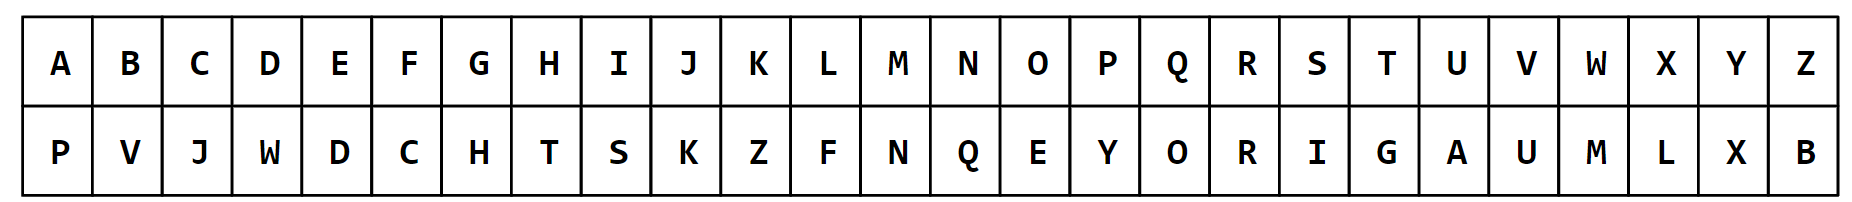
\includegraphics[scale=0.4]{../assets/simple_sub.png}
\end{center}
This tells us that 
\begin{itemize}
    \item to \emph{encrypt}, we just need to convert every instance of the top letter to the corresponding bottom letter. For example, encrypting $A$ becomes $P$, encrypting $B$ becomes $V$, and so on.
    \item to \emph{decrypt}, we just need to convert every instance of the bottom letter to the corresponding top letter. For example, decrypting $P$ becomes $A$, decrypting $V$ becomes $B$, and so on.
\end{itemize}
\begin{mdframed}
    (Example.) Suppose Alice wants to encrypt the message \code{You must destroy all of the horcruxes!} She starts by encoding the message\footnote{Removing all spaces, punctuations, and then capitalizing everything.}:
    \begin{verbatim}
YOUMUSTDESTRYALLOFTHEHORCRUXES\end{verbatim}
    Then, she converts each letter using the table: 
    \begin{verbatim}
XEANAIGWDIGREXPFFECGTDTERJRALDI\end{verbatim}
        This is the ciphertext she sends to Bob. To decrypt the message, Bob uses the same table backwards.
\end{mdframed}

Notice that, if the entire table is our key, the number of possible keys is $26!$, a \emph{huge} number. Despite this, simple substitution can still be broken relatively easily using some ideas from probability theory. 

\begin{mdframed}
    (Exercise.) Using the same table given above, do the following by hand. 

    \begin{enumerate}[(a)]
        \item Encrypt the message \code{The moon is pitted with holes!}
        \begin{mdframed}
            Encoding the message gives \code{THEMOONISPITTEDWITHHOLES}. Then, we just need to map each letter appropriately. 
            \begin{verbatim}
plaintext  T H E M O O N I S P I T T E D W I T H H O L E S
ciphertext G T D N E E Q S I Y S G G D W M S G T T E F D I\end{verbatim}
            The answer is \code{GTDNEEQSIYSGGDWMSGTTEFDI}.
        \end{mdframed}

        \item Decrypt the message \code{TEMPRDXEAWESQHGEWPX}.
        \begin{mdframed}
            Mapping each letter appropriately gives us
            \begin{verbatim}
ciphertext T E M P R D X E A W E S Q H G E W P X
plaintext  H O W A R E Y O U D O I N G T O D A Y\end{verbatim}
            Which, decoded, gives us \code{How are you doing today?}
        \end{mdframed}
    \end{enumerate}
\end{mdframed}



\subsection{Polybius Square}
The \textbf{Polybius Square} is another simple substitution cipher which replaces each letter of the plaintext with \emph{two} letters of ciphertext. The idea behind a Polybius square is that it's a table with labeled rows and columns; the alphabet for the messages we're encrypting lives inside the table. For example, if the alphabet we're encrypting includes the capital letters \code{A} through \code{Z} and the digits \code{0} through \code{9}, then we have 36 letters -- perfectly enough to fit in a $6 \times 6$ grid. Consider the following arrangement, using the rows and columns \code{ADFGVX}:
\begin{center}
    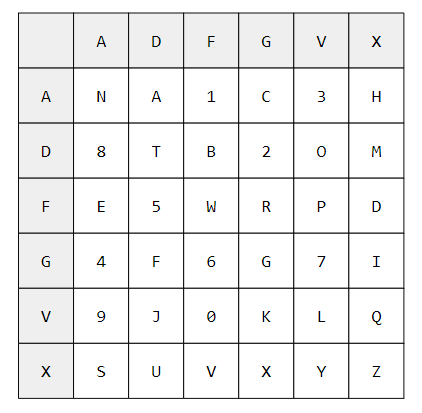
\includegraphics[scale=0.9]{../assets/polybius.png}
\end{center}
This table represents our key. To encrypt a message, we convert each letter in the plaintext to a pair of letters indicating the \emph{row} and \emph{column} of that letter in the table above. For example, \code{K} would be replaced with \code{VG}. Similarly, \code{S} would be replaced with \code{XA}. 

\begin{mdframed}
    (Example.) Suppose Alice wants to encrypt the message 
    \begin{verbatim}
Storm the gates at 14:37.\end{verbatim}
    She begins by encoding the message: 
    \begin{verbatim}
STORMTHEGATESAT1437\end{verbatim}
    Then, she goes through and replaces each letter by the corresponding pairs as described above:
    \begin{verbatim}
XADDDVFGDXDDAXFAGGADDDFAXAADDDAFGAAVGV\end{verbatim}
    This is the ciphertext. Bob, who knows the table, can undo this process to decrypt the message. 
\end{mdframed}

\begin{mdframed}
    (Exercise.) Use the square given above.
    \begin{enumerate}[(a)]
        \item Encrypt the message \code{Hide tide at 7:01am}.
        \begin{mdframed}
            Encoding the message gives us \code{HIDETIDEAT701AM}. Then, we can map each individual character in the plaintext to its ciphertext representation:
            \begin{center}
                \begin{tabular}{c|c}
                    \textbf{Plain} & \textbf{Cipher} \\ 
                    \hline 
                    H              & AX \\
                    I              & GX \\
                    G              & GG \\
                    H              & AX \\
                    T              & DD \\
                    I              & GX \\
                    D              & FX \\
                    E              & FA \\
                    A              & AD \\
                    T              & DD \\
                    7              & GV \\
                    0              & VF \\
                    1              & AF \\
                    A              & NN \\
                    M              & DX 
                \end{tabular}
            \end{center}
            Combining all of this gives us 
            \begin{mdframed}
                \begin{verbatim}
AXGXGGAXDDGXFXFAADDDGVVFAFNNDX\end{verbatim}
            \end{mdframed}
        \end{mdframed}
        \item Decrypt the message \code{XAAAADVGFAFVADDDAXADDDDGFVDX}.
        \begin{mdframed}
            To decrypt, we can map each pair of characters in the ciphertext to its plaintext representation:
            \begin{center}
                \begin{tabular}{c|c}
                    \textbf{Cipher} & \textbf{Plain} \\ 
                    \hline 
                    XA              & S \\
                    AA              & N \\
                    AD              & A \\
                    VG              & K \\
                    FA              & E \\
                    FV              & P \\
                    AD              & A \\
                    DD              & T \\
                    AX              & H \\
                    AD              & A \\
                    DD              & T \\
                    DG              & 2 \\
                    FV              & P \\
                    DX              & M 
                \end{tabular} 
            \end{center}
            Combining and decoding gives us 
            \begin{mdframed}
                \begin{verbatim}
Snake path at 2pm\end{verbatim}
            \end{mdframed}
        \end{mdframed}
    \end{enumerate}
\end{mdframed}

\end{document}